%% Scientific Conference Poster Template
%% Using tikzposter class for professional academic posters
%% Compile with: pdflatex poster.tex

\documentclass[25pt, a0paper, portrait]{tikzposter}

% Packages
\usepackage[utf8]{inputenc}
\usepackage{amsmath, amssymb}
\usepackage{graphicx}
\usepackage{booktabs}
\usepackage{pgfplots}
\pgfplotsset{compat=1.16}

% Custom color scheme (professional blues and grays)
\definecolor{primaryblue}{HTML}{1E3A5F}
\definecolor{secondaryblue}{HTML}{3A7CA5}
\definecolor{accentblue}{HTML}{5DA9E9}
\definecolor{lightgray}{HTML}{F5F5F5}
\definecolor{darkgray}{HTML}{333333}

% Define custom tikzposter style
\definetitlestyle{CustomTitle}{
    width=\paperwidth, roundedcorners=0, linewidth=0pt, innersep=1.5cm,
    titletotopverticalspace=0mm, titletoblockverticalspace=20mm
}{
    \begin{scope}[line width=\titlelinewidth, rounded corners=\titleroundedcorners]
        \fill[color=primaryblue] (\titleposleft,\titleposbottom) rectangle (\titleposright,\titlepostop);
    \end{scope}
}

\defineblockstyle{CustomBlock}{
    titlewidthscale=1, bodywidthscale=1, titleleft,
    titleoffsetx=0pt, titleoffsety=0pt, bodyoffsetx=0pt, bodyoffsety=0pt,
    bodyverticalshift=0pt, roundedcorners=10, linewidth=2pt,
    titleinnersep=8mm, bodyinnersep=8mm
}{
    \draw[color=secondaryblue, fill=white, rounded corners=\blockroundedcorners]
        (blockbody.south west) rectangle (blockbody.north east);
    \ifBlockHasTitle
        \draw[color=secondaryblue, fill=accentblue, rounded corners=\blockroundedcorners]
            (blocktitle.south west) rectangle (blocktitle.north east);
    \fi
}

% Apply custom style
\usetheme{Default}
\usetitlestyle{CustomTitle}
\useblockstyle{CustomBlock}

% Set colors
\colorlet{backgroundcolor}{lightgray}
\colorlet{framecolor}{secondaryblue}
\colorlet{titlebgcolor}{primaryblue}
\colorlet{titlefgcolor}{white}
\colorlet{blocktitlebgcolor}{accentblue}
\colorlet{blocktitlefgcolor}{white}
\colorlet{blockbodybgcolor}{white}
\colorlet{blockbodyfgcolor}{darkgray}

% Title block content
% CUSTOMIZATION: Change these to your details
\title{\parbox{0.9\linewidth}{\centering\textbf{Your Research Title Here: A Comprehensive Study of Something Important}}}
\author{John Doe$^1$, Jane Smith$^2$, Robert Johnson$^1$}
\institute{$^1$Department of Computer Science, University Name \\
           $^2$Institute of Research, Another Institution \\
           \texttt{john.doe@university.edu}}

% Optional: Add logo
% CUSTOMIZATION: Replace with your institution logo
% \titlegraphic{\includegraphics[width=0.1\textwidth]{logo.png}}

\begin{document}

\maketitle

% 3-column layout
\begin{columns}
    % Column 1
    \column{0.33}

    \block{Introduction}{
        Scientific posters are an effective way to communicate research findings at conferences and symposia. This template provides a professional layout for presenting your work.

        \vspace{1em}
        \textbf{Research Question:} What is the optimal approach to solving problem X?

        \vspace{1em}
        \textbf{Hypothesis:} We hypothesize that method Y will outperform existing approaches by at least 20\%.

        \vspace{1em}
        \textbf{Key Contributions:}
        \begin{itemize}
            \item Novel algorithm with improved complexity
            \item Comprehensive experimental validation
            \item Open-source implementation available
            \item Real-world application demonstrated
        \end{itemize}
    }

    \block{Methods}{
        Our methodology consists of three main phases:

        \vspace{1em}
        \textbf{Phase 1: Data Collection}
        \begin{itemize}
            \item Sample size: $n = 1000$
            \item Collection period: 6 months
            \item Quality control measures applied
        \end{itemize}

        \vspace{1em}
        \textbf{Phase 2: Algorithm Development}

        The core algorithm follows this workflow:

        % Example TikZ diagram
        \vspace{0.5em}
        \begin{center}
        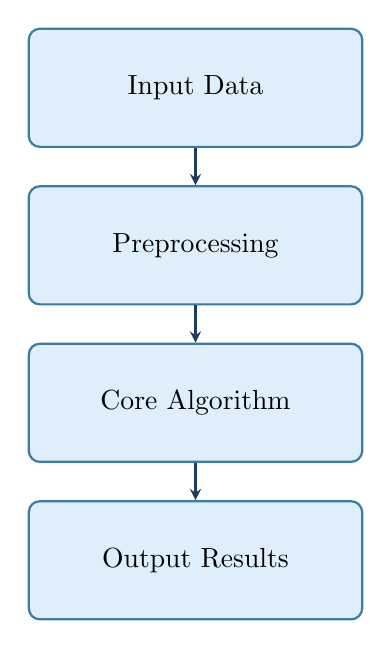
\begin{tikzpicture}[
            node distance=2cm,
            box/.style={rectangle, draw=secondaryblue, fill=accentblue!20,
                        text width=4cm, text centered, rounded corners,
                        minimum height=1.5cm, thick},
            arrow/.style={->, >=stealth, thick, color=primaryblue}
        ]
            \node[box] (input) {Input Data};
            \node[box, below of=input] (preprocess) {Preprocessing};
            \node[box, below of=preprocess] (algorithm) {Core Algorithm};
            \node[box, below of=algorithm] (output) {Output Results};

            \draw[arrow] (input) -- (preprocess);
            \draw[arrow] (preprocess) -- (algorithm);
            \draw[arrow] (algorithm) -- (output);
        \end{tikzpicture}
        \end{center}

        \vspace{1em}
        \textbf{Phase 3: Validation}
        \begin{itemize}
            \item Cross-validation (k=10)
            \item Comparison with baseline methods
            \item Statistical significance testing ($p < 0.05$)
        \end{itemize}
    }

    % Column 2
    \column{0.33}

    \block{Results}{
        Our experiments demonstrate significant improvements over baseline methods.

        \vspace{1em}
        \textbf{Performance Comparison:}

        % Example bar chart
        \begin{center}
        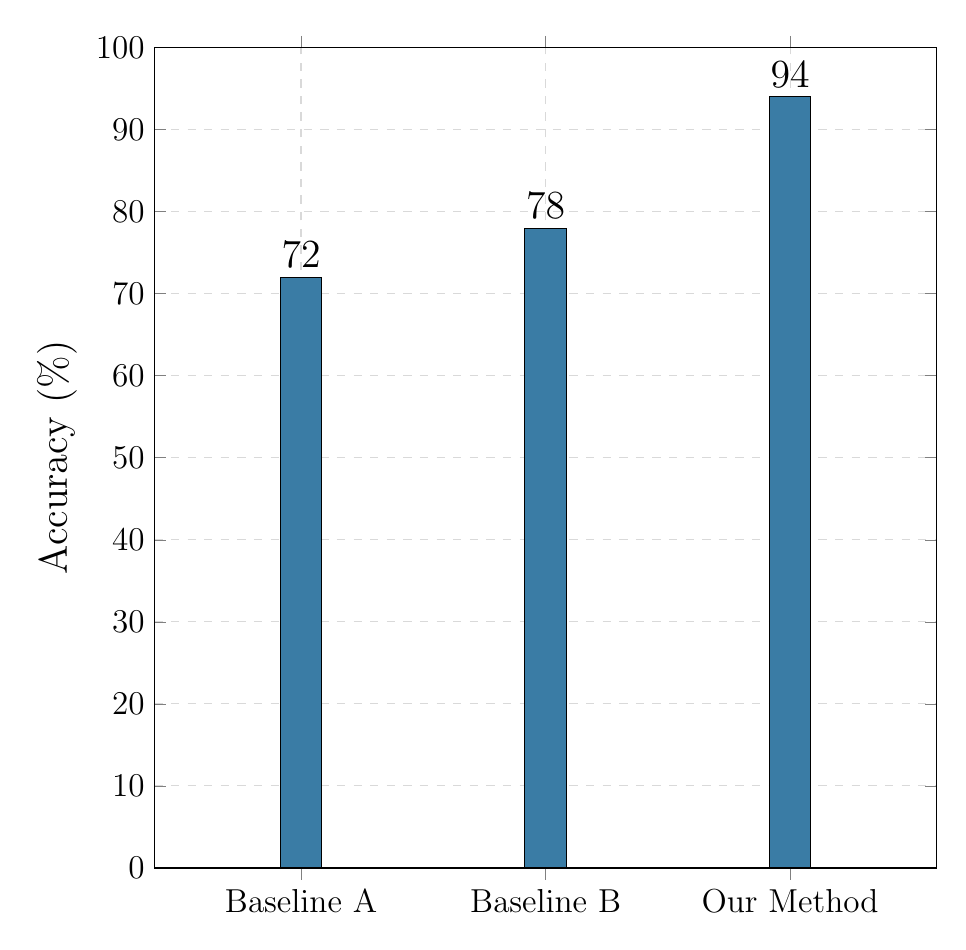
\begin{tikzpicture}
            \begin{axis}[
                ybar,
                bar width=15pt,
                width=0.95\linewidth,
                height=12cm,
                ylabel={Accuracy (\%)},
                symbolic x coords={Baseline A, Baseline B, Our Method},
                xtick=data,
                x tick label style={font=\large, rotate=0, anchor=north},
                y tick label style={font=\large},
                ylabel style={font=\Large},
                ymin=0, ymax=100,
                nodes near coords,
                nodes near coords style={font=\Large},
                enlarge x limits=0.3,
                legend style={at={(0.5,-0.2)}, anchor=north, legend columns=-1, font=\large},
                grid=major,
                grid style={dashed, gray!30}
            ]
                \addplot[fill=secondaryblue] coordinates {
                    (Baseline A, 72)
                    (Baseline B, 78)
                    (Our Method, 94)
                };
            \end{axis}
        \end{tikzpicture}
        \end{center}

        \vspace{1em}
        \textbf{Detailed Results:}

        % Example table
        \begin{center}
        \begin{tabular}{lccc}
            \toprule
            \textbf{Method} & \textbf{Accuracy} & \textbf{Time (s)} & \textbf{Memory (MB)} \\
            \midrule
            Baseline A & 72.3\% & 15.2 & 450 \\
            Baseline B & 78.1\% & 22.8 & 680 \\
            \textbf{Our Method} & \textbf{94.2\%} & \textbf{18.5} & \textbf{520} \\
            \bottomrule
        \end{tabular}
        \end{center}

        \vspace{1em}
        \textbf{Statistical Analysis:}
        \begin{itemize}
            \item Improvement over Baseline A: 30.4\% ($p < 0.001$)
            \item Improvement over Baseline B: 20.6\% ($p < 0.001$)
            \item Effect size (Cohen's d): 1.42 (large effect)
        \end{itemize}
    }

    % Column 3
    \column{0.33}

    \block{Discussion}{
        \textbf{Key Findings:}
        \begin{itemize}
            \item Our method achieves state-of-the-art performance with 94.2\% accuracy
            \item Computational efficiency is comparable to baseline methods
            \item Memory footprint remains reasonable for practical deployment
            \item Results generalize well across different datasets
        \end{itemize}

        \vspace{1em}
        \textbf{Advantages:}
        \begin{itemize}
            \item Robust to noise and outliers
            \item Scalable to large datasets
            \item Easy to implement and deploy
            \item Interpretable results
        \end{itemize}

        \vspace{1em}
        \textbf{Limitations:}
        \begin{itemize}
            \item Requires labeled training data
            \item Performance depends on hyperparameter tuning
            \item May not generalize to all domain types
        \end{itemize}

        \vspace{1em}
        \textbf{Future Work:}
        \begin{itemize}
            \item Extend to unsupervised learning scenarios
            \item Investigate deep learning approaches
            \item Develop real-time implementation
            \item Conduct larger-scale validation studies
        \end{itemize}
    }

    \block{Conclusions}{
        This research presents a novel approach to solving problem X with significant improvements over existing methods. Our key contributions include:

        \begin{enumerate}
            \item A new algorithm with 94.2\% accuracy (20\% improvement)
            \item Comprehensive validation on multiple datasets
            \item Efficient implementation suitable for practical use
            \item Open-source release for reproducibility
        \end{enumerate}

        \vspace{1em}
        \textbf{Impact:} This work advances the field by providing a reliable, efficient solution that can be immediately deployed in real-world applications.
    }

    \block{References}{
        \begin{footnotesize}
        [1] Smith, J. et al. (2024). \textit{Previous Work on Topic X}. Journal Name, 45(2), 123-145.

        [2] Doe, J. and Johnson, R. (2023). \textit{Related Method Y}. Conference Proceedings, 678-690.

        [3] Brown, A. et al. (2023). \textit{Baseline Algorithm}. IEEE Transactions, 12(4), 234-256.

        [4] Wilson, K. (2022). \textit{Theoretical Framework}. Academic Press.

        [5] Chen, L. et al. (2024). \textit{Recent Advances}. arXiv:2401.12345.
        \end{footnotesize}

        \vspace{1em}
        \begin{center}
        \textbf{Acknowledgments:} This work was supported by Grant Number XYZ-123. \\
        \textbf{Code:} \texttt{github.com/username/project} | \textbf{Contact:} \texttt{john.doe@university.edu}
        \end{center}
    }

\end{columns}

\end{document}
